% Asset ID: FAS1ConicSections1TikZ-002
% Source: FP1-Chp2-ConicSections1.pdf rectangular hyperbola summary
% Purpose: Precise labelled diagram of the rectangular hyperbola xy = c^2.
\documentclass[tikz,border=6pt]{standalone}
\usepackage{amsmath}
\usepackage{xcolor}
\usetikzlibrary{arrows.meta,calc,backgrounds}
\definecolor{canvas}{HTML}{FAF9F6}
\definecolor{ivory}{HTML}{FFFFF0}
\definecolor{linegray}{HTML}{E5E5EA}
\definecolor{gold}{HTML}{C5A059}
\definecolor{ink}{HTML}{2C2C2E}
\definecolor{rose}{HTML}{FBEFEF}
\definecolor{teal}{HTML}{6B9FA3}
\definecolor{purple}{HTML}{8F6C9F}
\begin{document}
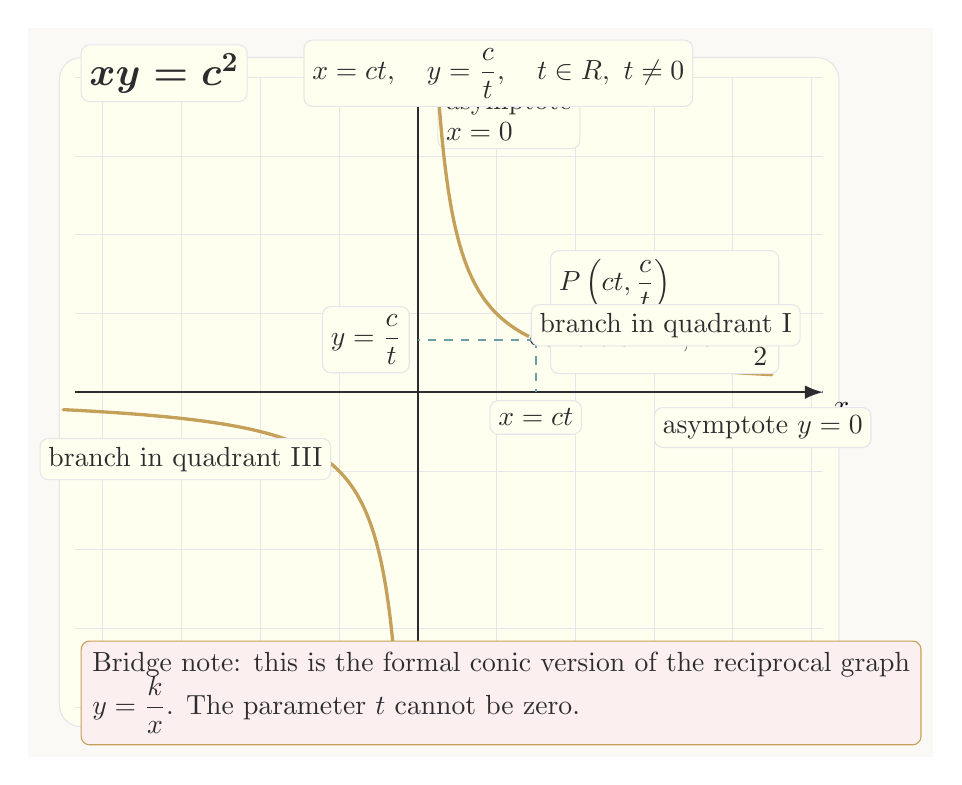
\begin{tikzpicture}[x=1cm,y=1cm,>=Latex,background rectangle/.style={fill=canvas},show background rectangle,
axis/.style={->,thick,draw=ink},gridline/.style={draw=linegray,line width=0.25pt},curve/.style={draw=gold,very thick,line cap=round},asymptote/.style={draw=purple,thick,dashed},guide/.style={draw=teal,thick,dashed},point/.style={circle,fill=ink,draw=ivory,line width=0.6pt,inner sep=1.7pt},labelbox/.style={fill=ivory,draw=linegray,rounded corners=3pt,inner sep=3pt,align=left,text=ink},warnbox/.style={fill=rose,draw=gold,rounded corners=3pt,inner sep=4pt,align=left,text=ink}]
\fill[ivory,rounded corners=8pt,draw=linegray] (-4.55,-4.25) rectangle (5.35,4.25);
\foreach \x in {-4,-3,...,5}{\draw[gridline] (\x,-4)--(\x,4);}
\foreach \y in {-4,-3,...,4}{\draw[gridline] (-4.35,\y)--(5.15,\y);}
\draw[asymptote] (0,-4)--(0,4); \draw[asymptote] (-4.35,0)--(5.15,0);
\draw[axis] (-4.35,0)--(5.15,0) node[below right] {$x$};
\draw[axis] (0,-4)--(0,4) node[above left] {$y$};
\node[labelbox,anchor=west] at (0.25,3.5) {asymptote\\[-1pt] $x=0$};
\node[labelbox,anchor=west] at (3.0,-0.45) {asymptote $y=0$};
\draw[curve,domain=0.25:4.5,samples=160,smooth,variable=\x] plot ({\x},{1/\x});
\draw[curve,domain=-4.5:-0.25,samples=160,smooth,variable=\x] plot ({\x},{1/\x});
\coordinate (P) at (1.5,0.6667);
\node[point] at (P) {};
\node[labelbox,anchor=west] at ($(P)+(0.18,0.35)$) {$P\left(ct,\dfrac{c}{t}\right)$\\[-1pt] here $c=1,\ t=\dfrac32$};
\draw[guide] (P)--(1.5,0); \draw[guide] (P)--(0,0.6667);
\node[labelbox,anchor=north] at (1.5,-0.1) {$x=ct$};
\node[labelbox,anchor=east] at (-0.1,0.6667) {$y=\dfrac{c}{t}$};
\node[labelbox] at (3.15,0.85) {branch in quadrant I};
\node[labelbox] at (-2.95,-0.85) {branch in quadrant III};
\node[labelbox,anchor=west] at (-4.28,4.05) {\Large $\boldsymbol{xy=c^2}$};
\node[labelbox,anchor=west] at (-1.45,4.05) {$x=ct,\quad y=\dfrac{c}{t},\quad t\in\mathbb{R},\ t\ne0$};
\node[warnbox,anchor=west] at (-4.28,-3.82) {Bridge note: this is the formal conic version of the reciprocal graph\\[-1pt] $y=\dfrac{k}{x}$. The parameter $t$ cannot be zero.};
\end{tikzpicture}
\end{document}
